\chapter{Methodology}

Anomaly detection in datasets containing AIS messages, as performed in this work, follows several steps involving data engineering techniques such as data cleaning, data normalization, and data transformation.
\\
The first step was data cleaning of the original data to avoid syntactic errors in the data. Then, an algorithm capable of generating the "trip" entities from the individual messages was developed, since the trip is the selected entity for the clustering. In a third step, all numerical chosen features were associated with each trip in order to enable a distance-based clustering algorithm such as \textbf{DBScan}.

\section{Data cleaning and normalization}
    In order to better manage and detect anomalies, a data cleaning task was performed as preliminary steps.
    Indeed, it is likely that an error has occurred in the recording or acquisition of data, resulting in a syntactically anomalous register of information. This has resulted in some isolated records in the dataset that would be better corrected or removed before proceeding with anomaly detection.
    \\
    Corrupt records in data set fall into the following categories:
    \begin{itemize}
        \item Messages coming from ships without an appropriate identifier.
        \\
        This would have made it difficult to assign the message to a specific ship and thus to a voyage. Messages with the value '0' as \verb|mmsi| (the ship identifier used in this work) and with 'UNAVAILABLE' as \verb|vessel_name| were accordingly removed before we proceeded to the next steps.
        
        \item Messages with coordinates that correspond to land and not to a maritime area.
        In order to properly achieve this goal, the python packages \underline{\href{https://scitools.org.uk/cartopy/docs/latest/}{cartopy}} by scitools and \underline{\href{https://shapely.readthedocs.io/en/stable/manual.html}{shapely}} has been used to detect anomaly coordinates to remove them from the data set.
        
        
        \begin{minipage}{\linewidth}
        \begin{lstlisting}[language=Python]

import cartopy.io.shapereader as shpreader
import shapely.geometry as sgeom
from shapely.ops import unary_union
from shapely.prepared import prep

# defining the shape of area of earth
# with a resolution of 10m
land_shp_fname = shpreader.natural_earth(
    resolution='10m', 
    category='physical', 
    name='land')
#join all the land polygons together
land_geom = unary_union(
    list(shpreader.Reader(land_shp_fname).geometries()))
land = prep(land_geom)

# defining function is_land
# param msg is the tuple of the message
# return boolean if the messgae was sent from a land point
def is_land(msg):
    return land.contains(
        sgeom.Point(
            msg['longitude'], msg['latitude']))
    
        \end{lstlisting}
        
        \begin{figure}[H]
            \centering
            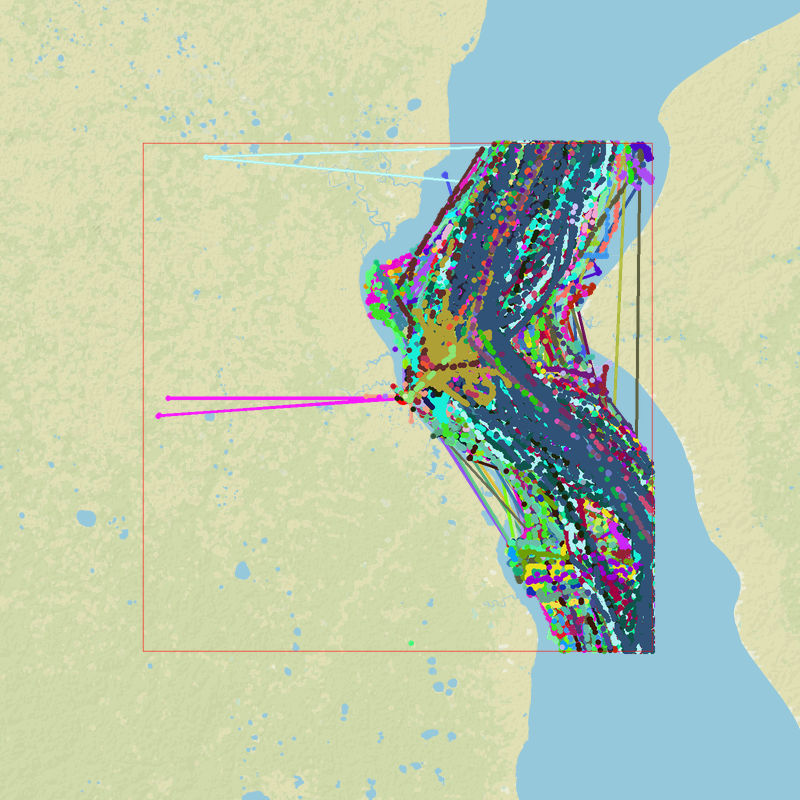
\includegraphics[width=9cm]{Images/land-points.png}
            \caption{Presence of wrong vessel coordinates on land}
        \end{figure}
        
        \end{minipage}
        
    \end{itemize}

        
    In addition, some normalization work was done on the data set.
    \\
    At the moment, all the information about the ship from which the message arrived is contained in the message record. This setting, in addition to weighing down the dataset considerably due to a huge amount of redundant data (12 fields out of 33 contain information about the ship and not the message) opens the possibility of inconsistent information.
    \\
    
    \begin{tabular}{|c|c|c|c|c|c|}
        \hline
            \textbf{index} & \textbf{imo} & \textbf{vessel\_name} & \textbf{callsign} & \textbf{vessel\_type} & \textbf{vessel\_class} \\
        \hline
            \textbf{5085} & 9120293      & KAPITAN BACHURIKHIN   & UDIZ              & Fishing               & \textcolor{red}{B}      \\
            \textbf{5086} & 9120293      & KAPITAN BACHURIKHIN   & UDIZ              & Fishing               & \textcolor{red}{A}      \\
        \hline
    \end{tabular}
    \\
    
    Above there is an example of data inconsistency messages 5085 and 5086 comes both from the same vessel but the class registered is different.
    \\
    This is impossible since the class is a vessel-related information.
    
    % PARLARE DELLA NORMALIZZAZIONE
    
    \bigbreak
    
    \begin{tabular}{|c|c|c|c|c|c|}
        \hline
            \textbf{index} & \textbf{imo} & \textbf{vessel\_name} & \textbf{callsign} & \textbf{vessel\_type} & \textbf{vessel\_class} \\
        \hline
            \textbf{31699} & 66550      & \textcolor{red}{OTA-883 *!0}   & UDIZ              & Reserved               & A      \\
            \textbf{31699} & 66550      & \textcolor{red}{OTA-883}   & UDIZ              & Reserved               & A      \\
        \hline
    \end{tabular}

\clearpage
\section{Trip Generation}

    As mentioned above, the object of analysis for anomaly detection is the entities \textbf{trips}. These are will be associated with numerical features useful for performing distance-based clustering such as DBScan. With the current state of the data, there is no deterministic way to cluster messages by trip (e.g., a trip\_id field in the message dataset).
    \\
    Therefore, it is necessary to define the concept of a trip and write an algorithm that can determine, under certain rules, to which trip each message belongs.
    \\
    The algorithm begins by sorting the receipt of messages chronologically for each ship and performs a scrolling of messages to allow grouping along the way.
    When scrolling through the messages in chronological order, the messages were associated to a trip entity. Doing that, the following factors caused it to be interrupted and a new one to be created.
    
    \begin{itemize}
    
    \item A time frame of more then \verb|SEGMENTS_MAX_DELTA_SECONDS| seconds between two consecutive messages. This variable specifies the minimum time interval between a message A and the next message B, sufficient to consider the two messages as belonging to two different trips. If this is the case, the sequence of successive messages is stopped and message B initiates a new sequence. This variable was given an arbitrary value of \textbf{86400 seconds} (24 hours)
    
    \item The arrival of a message with a change in the status of the ship to "moored". If the ship moors in a port but departs before \verb|SEGMENTS_MAX_DELTA_SECONDS| seconds have elapsed, the script considers two different trips that must be analyzed separately
    \end{itemize}
    \\
    
    \begin{minipage}{\linewidth}
    \begin{lstlisting}[language=Python]
coords = []
cur_coords = []
last_point = None
rows = load_vessel_file(file_path)
if len(rows) > 1:
    for row in rows:
        timestamp, latitude, longitude, status = row[0], row[1], row[2], row[3]
        # Check if is the first point
        if last_point is None:
             # check if the status is "moored"
            if status == 5:
                continue
            else:
                # register the first point
                cur_coords.append((timestamp, latitude, longitude))
        else:
            # check if the status is "moored"
            if status == 5:

                # get the last point status
                last_point_status = last_point[3]
                if last_point_status == 5:
                    pass
                else:
                    cur_coords.append((timestamp, latitude, longitude))
                    coords.append(cur_coords)
                    cur_coords = []
            else:
                delta_time = (timestamp - last_point[0])
                
                # check if the delta time is more then the max delta time
                if delta_time < settings.SEGMENTS_MAX_DELTA_TIMESTAMP_SECONDS:
                    cur_coords.append((timestamp, latitude, longitude))
                else:
                    if len(cur_coords) > 0:
                        coords.append(cur_coords)
                    cur_coords = [(timestamp, latitude, longitude)]

        last_point = (timestamp, latitude, longitude, status)
    if cur_coords:
        coords.append(cur_coords)
    \end{lstlisting}
    \end{minipage}

\section{Trip Features Association}
    One of the most important preliminary steps before applying the DBSCAN clustering method is by far the selection and computation of the \textbf{numerical features} that will become the dimensions we use to describe our entities in space.
     
    The selection of features is so important because the algorithm is able to consider trips as \textit{near} or \textit{far} from each other based on these features. Indeed, a correctly detected anomaly is one that highlights a value of some features that are substantially distant from a group of features with relatively similar values.
    
    Here are the selected trip features and how they were calculated:
    
    \subsubsection{min\_lat, max\_lat, min\_lon, max\_lon}
        These parameters are useful to describe the perimeter in which the ship moved during its voyage. Using these four features, the DBSCAN clustering algorithm can group voyages with trajectories in very similar areas.
    
    \subsubsection{start\_lat, start\_lon, end\_lat, end\_lon}
        These parameters are useful to describe the departure and arrival coordinates of the ship during the voyage. Using these four features, the DBSCAN clustering algorithm can group together voyages with similar departure and arrival points.
    
    \subsubsection{duration}
    
        This feature indicates the duration of the trip. Let \verb|ts_arr| be the array containing the timestamps of each message belonging to the trip. Duration in seconds is calculated as below:
        
        \begin{lstlisting}[language=Python, frame=none]
duration = max(ts_arr) - min(ts_arr)
        \end{lstlisting}
        
    \subsubsection{delay}
    
        Il ritardo maturato da una nave durante un viaggio potrebbe essere un ottimo parametro per evidenziare un'anomalia. Quest'ultimo viene calcolato grazie alla presenza del parametro eta (Estimated Time of Arrival) presente in ogni messaggio. A questo scopo si prende come riferimento il primo messaggio, quindi:
        
        \begin{lstlisting}[language=Python, frame=none]
delay = trip_msgs[0]['eta'] - duration
        \end{lstlisting} 
        
        \verb|delay < 0| $\rightarrow$ the vessel is the ship is ahead of schedule;
        \\
        \verb|delay > 0| $\rightarrow$ the vessel is late.
        
    \subsubsection{mean\_sog}
    
    As explained in the Data Description section, \textbf{sog} (Speed Over Ground) indicates the speed of the ship during its voyage. In order to point out anomalies such as excessive deceleration, this feature has been added and calculated as follows:
    
    \begin{lstlisting}[language=Python, frame=none]
mean_sog = np.array([x['sog'] for x in going_msgs]).mean()
    \end{lstlisting} 
    
    Note that \verb|going_msgs| is different from \verb|trip_msgs|, as the former only considers messages in which the ship is in \textit{Under Way Using Engine} state, making the calculation of these values more meaningful.
            
    \subsubsection{mean\_cog}
    
    The message parameter \textbf{cog}, which indicates the actual direction of motion taking into account compensation for wind and other flow forces, was chosen as trip feature because the average of this value over the entire trip might reveal some anomalies in the trajectory with respect to other similar trips.
    
    \begin{lstlisting}[language=Python, frame=none]
mean_sog = np.array([x['cog'] for x in going_msgs]).mean()
    \end{lstlisting} 
    
    \subsubsection{going\_time}
    
    
    
    \subsubsection{ideal\_distance}
    \subsubsection{actual\_distance}

\clearpage
\section{DBSCAN Clustering and Anomaly Detection}
    